\chapter{Theoretical Implementation}

\section{Dataset selection}
Which datasets are available?


\section{Business Understanding}

\section{Data Understanding}



\section{Data preparation}

\subsection{Data processing and data wrangling}
The data is available as a local folder of size 5.12 GB, it contains 152,592 \ac{JSON} files. Each \ac{JSON} represents one invoice document. 
	
For the data wrangling the invoices have to be read into memory and then processed into a reusable structure. Each document will be read into memory, then the necessary information will be extracted. All invoices will be combined into one data structure, which then is persisted for later use.

Explain the structure of one invoice.
Explain which data structures I want to use.

\begin{figure}[ht]
	\centering
	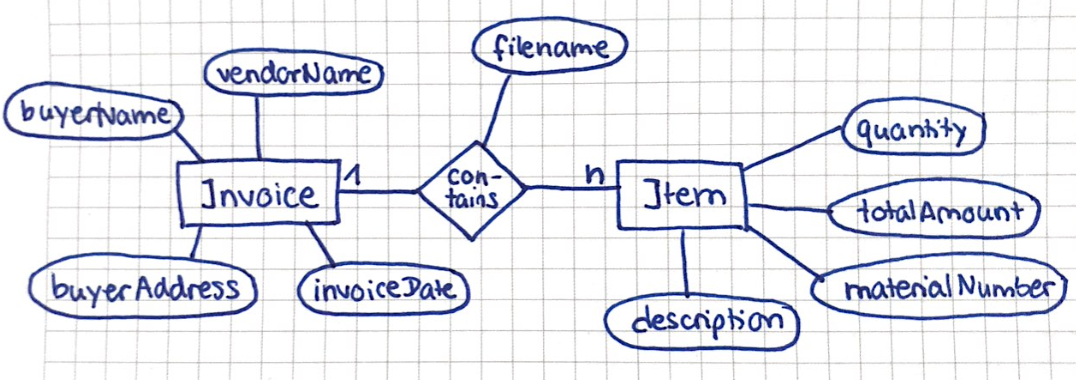
\includegraphics[height=5cm]{Bilder/practical/entity_relationship.png}
	\caption{Entity Relationship Diagram for Invoce Documents}
	\label{fig:er}
\end{figure}


Explain how I want to store the data. Explain the successive artifacts.

\subsection{Data cleaning}


\subsection{Feature Extraction and Feature Engineering}

\section{Modelling}
\section{Evaluation}
\subsection{Visualization}
\section{Deployment}